\documentclass[11pt,a4paper,reqno]{amsart}

\usepackage[utf8]{inputenc}
\usepackage[T1]{fontenc}
\usepackage{lmodern}
\usepackage{amsmath,amssymb,amsthm}
\usepackage{graphicx}
\usepackage[margin=28mm]{geometry}
\usepackage{xurl}
\usepackage[hidelinks]{hyperref}
\usepackage{orcidlink}
\usepackage{microtype}

\newtheorem{theorem}{Theorem}[section]
\newtheorem{lemma}[theorem]{Lemma}
\newtheorem{proposition}[theorem]{Proposition}
\newtheorem{corollary}[theorem]{Corollary}
\newtheorem{conjecture}{Conjecture}
\renewcommand{\theconjecture}{\Alph{conjecture}}
\theoremstyle{definition}
\newtheorem{definition}[theorem]{Definition}
\theoremstyle{remark}
\newtheorem{remark}[theorem]{Remark}

\newcommand{\cbar}[1]{\overline{C_{#1}}}
\newcommand{\df}{\operatorname{def}}
\hypersetup{pdftitle={Every odd antihole is strongly chromatic-choosable},pdfauthor={Deep Bhattacharjee, Ushashi Bhattacharya}}

\title[Every odd antihole is strongly chromatic-choosable]{Every odd antihole is strongly chromatic-choosable}

\author{Deep Bhattacharjee\,\orcidlink{0000-0003-0466-750X}}
\address{Formerly, Electro-Gravitational Space Propulsion Laboratory (EGSPL), Bhubaneswar, Odisha 751030, India}
\address{Formerly, University of Calcutta, Senate House, 87/1 College Street, Kolkata 700073, West Bengal, India}
\email{d.bhattacharjee@erl-forschung.de}
\email{itsdeep@live.com}
\email{egspl@proton.me}
\thanks{\sloppy Corresponding author: Deep Bhattacharjee. Email: \href{mailto:d.bhattacharjee@erl-forschung.de}{d.bhattacharjee@erl-forschung.de}, \href{mailto:itsdeep@live.com}{itsdeep@live.com}, \href{mailto:egspl@proton.me}{egspl@proton.me}; ORCID \href{https://orcid.org/0000-0003-0466-750X}{0000-0003-0466-750X}.}
\author{Ushashi Bhattacharya\,\orcidlink{0009-0002-2254-3914}}
\address{Formerly, National Taiwan University, Taipei 106319, Taiwan}
\email{rai.bhattacharya.in@gmail.com}
\thanks{Ushashi Bhattacharya: email \href{mailto:rai.bhattacharya.in@gmail.com}{rai.bhattacharya.in@gmail.com}; ORCID \href{https://orcid.org/0009-0002-2254-3914}{0009-0002-2254-3914}.}

\subjclass[2020]{05C15; 05C17; 05C38}
\keywords{list colouring; odd antihole; chromatic-choosability; critical graph}
\date{26 October 2026}

\begin{document}

\begin{abstract}
\itshape
A hole in a graph is an induced cycle of length at least four, and an antihole is the complement of a hole. Odd holes and odd antiholes are the graphs that, by the strong perfect graph theorem, force the chromatic number above the clique number. Fiujlaali and McDonald studied the odd antiholes inside $k$-critical graphs of maximum degree $\Delta$, proved that such an antihole has at most $2(\Delta-k)+7$ vertices, and conjectured that this bound is attained only when the graph is the antihole itself, provided the graph has no odd hole. They reduced this to a statement about list colouring: for every $\ell\ge3$, the odd antihole on $2\ell-1$ vertices has chromatic number $\ell$, and the only assignments of lists of $\ell-1$ colours from which it cannot be coloured are those in which all lists are equal. This is their Conjecture~9, and they proved it when all the lists lie in a common set of $\ell$ colours. We prove it for every $\ell$ with no restriction on the lists, and we deduce their Conjecture~3 for all $k$ and $\Delta$. The proof works with the complements of disjoint unions of paths with an odd number of vertices. The vertices in even positions of the paths form a clique in the complement, so equal lists of one colour fewer than the number of these vertices cannot be completed; we show by induction, using Hall's theorem and the theorem of Erd\H{o}s, Rubin and Taylor on complete multipartite graphs with parts of size at most two, that this is the only obstruction, and a separate lemma on minimal tight sets settles the extremal case of a single path. The cycle is then closed by carrying a colour shared by two consecutive vertices around the odd cycle in steps of two. The theorem also gives an infinite family of strongly chromatic-choosable graphs that are not strongly critical in the sense of Stiebitz, Tuza and Voigt. Every statement is proved by hand.
\end{abstract}

\maketitle



\medskip
\begin{quote}
\small\sloppy
\noindent\textbf{Note.} The results of this paper were first made public on 15 October 2026, as release \texttt{v1.0.0} of the repository \url{https://github.com/creelie/odd-antihole}, archived on Zenodo as \href{https://doi.org/10.5281/zenodo.23393861}{10.5281/zenodo.23393861}; later versions (\texttt{v1.1.0} of 21 October and \texttt{v1.2.0} of 26 October) are archived as \href{https://doi.org/10.5281/zenodo.23541224}{10.5281/zenodo.23541224} and \href{https://doi.org/10.5281/zenodo.23662269}{10.5281/zenodo.23662269} (concept DOI \href{https://doi.org/10.5281/zenodo.23393860}{10.5281/zenodo.23393860}). An earlier and incomplete version of the paper appeared on Hexagon on 17 October 2026 as the preprint \texttt{hexagon:2610.00319}, available at \url{https://hexagonmath.org/2610.00319}. That version carried a section on a machine verification of the main theorem and on computer checks of small cases, cited a release of the repository as a reference, and had a short abstract. This version is complete and self-contained: every statement is proved by hand in Sections~\ref{sec:prelim} to~\ref{sec:critical}, so that no statement rests on a computer, every reference has been checked at its source, and the abstract states what is proved. The source of this revision is in release \texttt{v2.0.0} of the same repository, archived as \href{https://doi.org/10.5281/zenodo.23663712}{10.5281/zenodo.23663712}, with programs that check the main theorem on the antiholes with five and seven vertices.
\end{quote}

\section{Introduction}

All graphs are finite and simple. A \emph{hole} is an induced cycle of length at least four and an \emph{antihole} is an induced copy of the complement $\cbar{t}$ of a cycle $C_t$ with $t\ge4$; holes and antiholes are \emph{odd} when $t$ is odd. By the Strong Perfect Graph Theorem of Chudnovsky, Robertson, Seymour and Thomas~\cite{CRST}, a graph whose chromatic number exceeds its clique number contains an odd hole or an odd antihole. Following Fiujlaali and McDonald~\cite{FM}, a graph $G$ is \emph{$k$-critical} if $\chi(G)=k$ and $\chi(G-v)<k$ for every vertex $v$.

Fiujlaali and McDonald~\cite{FM} study the odd antiholes in critical graphs of given maximum degree. They prove that every odd antihole in a $k$-critical graph of maximum degree $\Delta$ has length at most $2(\Delta-k)+7$, and they ask whether the bound is attained only by the antihole itself.

\begin{conjecture}[{\cite[Conjecture~3]{FM}}]\label{conj:3}
Let $G$ be an odd-hole-free $k$-critical graph with maximum degree $\Delta$. If $G$ contains an odd antihole of length $2(\Delta-k)+7$, then $G=\cbar{2(\Delta-k)+7}$.
\end{conjecture}

They prove Conjecture~\ref{conj:3} when $\Delta\le k$ and when $\Delta\ge2k-5$ \cite[Theorem~4]{FM}; the case $\Delta=k$ is a theorem of Chen, Lan, Lin and Zhou~\cite{CLLZ} and of Galindo, McDonald and Shan~\cite{GMS}. The range $k<\Delta<2k-5$ remained open, and its first case is $(k,\Delta)=(7,8)$.

The tool is list colouring. A \emph{list assignment} $L$ for a graph $G$ gives each vertex $v$ a finite set $L(v)$ of colours, and $G$ is \emph{$L$-colourable} if there is a proper colouring $f$ of $G$ with $f(v)\in L(v)$ for every $v$. An \emph{$m$-assignment} is a list assignment in which every list has exactly $m$ colours. Following Kaul and Mudrock~\cite{KM}, a graph $G$ is \emph{strongly $k$-chromatic-choosable} if $\chi(G)=k$ and every $(k-1)$-assignment $L$ for which $G$ is not $L$-colourable is constant, that is, $L(u)=L(v)$ for all vertices $u,v$. Fiujlaali and McDonald prove that $\cbar{2\ell-1}$ is $L$-colourable for every non-constant $(\ell-1)$-assignment whose lists lie in a common set of $\ell$ colours \cite[Theorem~8]{FM}, and they conjecture that the common set can be dropped.

\begin{conjecture}[{\cite[Conjecture~9]{FM}}]\label{conj:9}
For every integer $\ell\ge3$, the odd antihole $\cbar{2\ell-1}$ is strongly $\ell$-chromatic-choosable.
\end{conjecture}

They show that Conjecture~\ref{conj:9} for $\ell$ implies Conjecture~\ref{conj:3} for every pair $(k,\Delta)$ with $\Delta-k=\ell-4$ \cite[Theorem~10]{FM}. The case $\ell=3$ is the classical fact that an odd cycle with lists of size two can be coloured unless all lists are equal. We prove the conjecture for every $\ell$.

\begin{theorem}\label{thm:main}
For every integer $\ell\ge3$ the odd antihole $\cbar{2\ell-1}$ is strongly $\ell$-chromatic-choosable. More precisely, $\chi(\cbar{2\ell-1})=\ell$, and if $L$ is a list assignment for $\cbar{2\ell-1}$ in which every list has at least $\ell-1$ colours and $\cbar{2\ell-1}$ is not $L$-colourable, then all lists are one and the same set of $\ell-1$ colours.
\end{theorem}

\begin{corollary}\label{cor:conj3}
Conjecture~\ref{conj:3} holds: if $G$ is an odd-hole-free $k$-critical graph of maximum degree $\Delta$ and $G$ contains an odd antihole of length $2(\Delta-k)+7$, then $G$ is this antihole.
\end{corollary}

Theorem~\ref{thm:main} is a sharp form of Ohba's conjecture for odd antiholes. Ohba's conjecture, proved by Noel, Reed and Wu~\cite{NRW}, states that a $k$-chromatic graph with at most $2k+1$ vertices is $k$-choosable~\cite{Ohba}; $\cbar{2\ell-1}$ has $2\ell-1$ vertices and chromatic number $\ell$, so lists of size $\ell$ always suffice. Theorem~\ref{thm:main} says that lists of size $\ell-1$ suffice as well, unless they are all equal.

Strong chromatic-choosability is a relative of the strongly critical graphs of Stiebitz, Tuza and Voigt~\cite{STV}: a graph is \emph{strongly $k$-critical} if it is $k$-critical in the sense that every proper subgraph has smaller chromatic number, and every $(k-1)$-assignment from which it cannot be coloured is constant. Complete graphs, odd cycles, two further families of graphs on $2k-1$ vertices, and joins of strongly critical graphs with cliques are strongly critical~\cite{STV}, and Bernshteyn, Kaul, Mudrock and Sharma~\cite{BKMS} add joins of critical graphs with large cliques. For $\ell\ge4$ the antihole $\cbar{2\ell-1}$ is not among these graphs, and it is not strongly critical: if $v_0v_1\cdots v_{2\ell-2}v_0$ is the cycle, the vertices $v_0$ and $v_3$ have no common neighbour on it, so after the edge $v_0v_3$ is removed from $\cbar{2\ell-1}$ every colour class still has at most two vertices, and the chromatic number is still $\ell$.\footnote{Every graph in the two families of~\cite{STV} on $2k-1$ vertices has a vertex of degree $k-1$, whereas $\cbar{2\ell-1}$ is regular of degree $2\ell-4>\ell-1$ for $\ell\ge4$. The antihole is not a join, since its complement $C_{2\ell-1}$ is connected.} Theorem~\ref{thm:main} therefore gives an infinite family of strongly chromatic-choosable graphs that are not strongly critical; Kaul and Mudrock~\cite{KM} and Bernshteyn, Kaul, Mudrock and Sharma~\cite{BKMS} give other such graphs.

\subsection*{The proof}
A colour class of $\cbar{2\ell-1}$ is a clique of $C_{2\ell-1}$, so it is a single vertex or two consecutive vertices of the cycle. Removing two consecutive vertices from the cycle leaves a path, so the proof turns on colourings of complements of paths, and more generally of disjoint unions of paths with an odd number of vertices. On such a union we call the vertices in even positions of each path \emph{outer}. If there are $s$ outer vertices, they form a clique of size $s$ in the complement, so constant lists of size $s-1$ on the outer vertices cannot be completed to a colouring. Theorem~\ref{thm:path} shows that, for lists of size at least $s-1$, this is the only obstruction, whatever the lists of the other vertices are. The proof is an induction on the number of vertices, driven by Hall's theorem and by the choosability of complete multipartite graphs with parts of size at most two (Lemma~\ref{lem:ert}); the extremal case, a single path with $2k$ colours in all, is settled separately in Lemma~\ref{lem:key}. Theorem~\ref{thm:cycle} then closes the cycle: if two consecutive vertices share a colour $c$, the path theorem applied to the rest of the cycle with $c$ removed propagates $c$ and the lists around the cycle in steps of two, and since the cycle is odd these steps reach every vertex. Figure~\ref{fig:roadmap} shows the order of the argument. Section~\ref{sec:critical} deduces Corollary~\ref{cor:conj3} by the argument of Fiujlaali and McDonald. Every step is a finite counting argument, of the same kind as the counts attached to finite complexes and group actions in the authors' earlier work~\cite{Bha22a,Bha22b,BB26}.

\begin{figure}[ht]
\centering
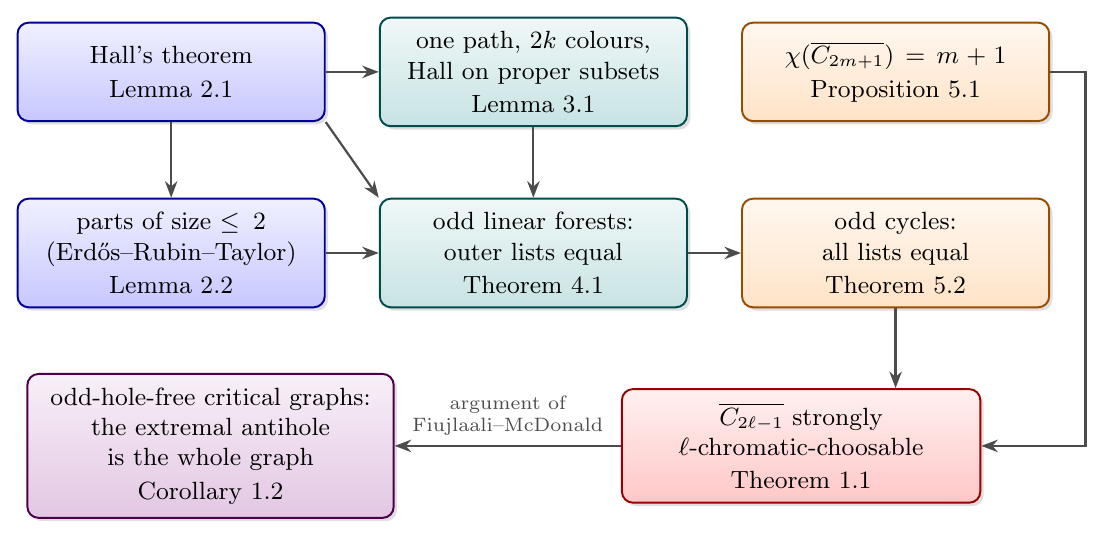
\includegraphics[width=0.92\textwidth]{figures/fig_roadmap.png}
\caption{The order of the proof. Arrows point from a result to the results that use it.}
\label{fig:roadmap}
\end{figure}


\section{Colourings of complements}\label{sec:prelim}

Throughout, $H$ is a graph with vertex set $V$ and $L$ is a list assignment on $V$. An \emph{$L$-colouring of the complement} $\overline H$ is a map $f$ with $f(v)\in L(v)$ for every $v\in V$ such that two distinct vertices receive the same colour only if they are adjacent in $H$. For $W\subseteq V$ we write
\[
L(W)=\bigcup_{w\in W}L(w),\qquad \df(W)=|W|-|L(W)|,
\]
so that $\df(\varnothing)=0$. The complement of an induced subgraph $H[X]$ is the induced subgraph $\overline H[X]$, and we use this without comment. We use Hall's theorem~\cite{Hall} in the following form.

\begin{lemma}\label{lem:hall}
If $|L(W)|\ge|W|$ for every $W\subseteq V$, then there is an injective map $f$ on $V$ with $f(v)\in L(v)$ for every $v$. Such a map is an $L$-colouring of $\overline H$ for every graph $H$ on $V$.
\end{lemma}

The next lemma is the theorem of Erd\H{o}s, Rubin and Taylor~\cite{ERT} that complete multipartite graphs whose parts have at most two vertices are chromatic-choosable. We include the short proof, since the same counting returns in Sections~\ref{sec:key} and~\ref{sec:cycle}.

\begin{lemma}\label{lem:ert}
Let $q\ge0$, and suppose that $V$ is the union of at most $q$ pairwise disjoint sets, each of which is a single vertex or the two ends of an edge of $H$. If $|L(v)|\ge q$ for every $v\in V$, then $\overline H$ is $L$-colourable.
\end{lemma}

\begin{proof}
We use induction on $q$. If $q=0$ then $V$ is empty. Let $q\ge1$. Suppose first that some part $\{x,y\}$ has a colour $c\in L(x)\cap L(y)$. Give $c$ to $x$ and to $y$, and remove $c$ from the lists of the other vertices. The remaining vertices are covered by at most $q-1$ parts and their lists keep at least $q-1$ colours, so by induction they can be coloured. Since $xy$ is an edge of $H$ and no other vertex uses $c$, the result is an $L$-colouring of $\overline H$.

Otherwise the two lists of each part are disjoint, so each colour lies in the lists of at most one vertex of each part, and hence in at most $q$ lists. For $W\subseteq V$, counting pairs $(w,c)$ with $w\in W$ and $c\in L(w)$ gives
\[
q|W|\le\sum_{w\in W}|L(w)|\le q\,|L(W)|,
\]
so $|L(W)|\ge|W|$, and Lemma~\ref{lem:hall} applies.
\end{proof}

\section{The key lemma}\label{sec:key}

This section treats a single path with an odd number of vertices in the extremal situation that arises in the proof of Theorem~\ref{thm:path}.

\begin{lemma}\label{lem:key}
Let $k\ge1$, let $P=v_0v_1\cdots v_{2k}$ be a path with vertex set $V$, and let $L$ be a list assignment with $|L(v)|\ge k$ for every $v\in V$, with $|L(V)|=2k$, and with $|L(W)|\ge|W|$ for every $W\subsetneq V$. If $\overline P$ is not $L$-colourable, then $L(v_j)\cap L(v_{j+1})=\varnothing$ for $0\le j<2k$. Consequently every list has exactly $k$ colours and $L(v_0)=L(v_2)=\dots=L(v_{2k})$.
\end{lemma}

\begin{proof}
Suppose that $\overline P$ is not $L$-colourable. Call a nonempty set $W\subsetneq V$ \emph{tight} if $|L(W)|\le|W|$; by hypothesis a tight set satisfies $|L(W)|=|W|$. A tight set is \emph{minimal} if no proper nonempty subset of it is tight.

\smallskip\noindent(a) \emph{For every $x\in V$ there is a minimal tight set not containing $x$.} The set $V\setminus\{x\}$ is nonempty, and it is tight because $|L(V\setminus\{x\})|\le|L(V)|=2k=|V\setminus\{x\}|$. A tight subset of $V\setminus\{x\}$ of least size is minimal.

\smallskip\noindent(b) \emph{Matchings that avoid one vertex.} For $x\in V$, every subset of $V\setminus\{x\}$ is a proper subset of $V$, so Lemma~\ref{lem:hall} gives an injective map $\varphi_x$ on $V\setminus\{x\}$ with $\varphi_x(v)\in L(v)$. If $W$ is tight and $x\notin W$, then $\varphi_x(W)\subseteq L(W)$ and $|\varphi_x(W)|=|W|\ge|L(W)|$, so $\varphi_x(W)=L(W)$. By injectivity,
\begin{equation}\label{eq:outside}
\varphi_x(v)\notin L(W)\quad\text{for every }v\in V\setminus(W\cup\{x\}).
\end{equation}

\smallskip\noindent(c) \emph{A shared colour across the boundary of a minimal tight set gives a colouring.} Let $W$ be a minimal tight set, and let $x\notin W$ and $y\in W$ be adjacent in $P$ with a common colour $c\in L(x)\cap L(y)$. A nonempty set $Y\subseteq W\setminus\{y\}$ is a proper subset of $W$, so it is not tight and $|L(Y)|\ge|Y|+1$; hence $|L(Y)\setminus\{c\}|\ge|Y|$. By Lemma~\ref{lem:hall} there is an injective map $g$ on $W\setminus\{y\}$ with $g(v)\in L(v)\setminus\{c\}$. Put
\[
f(x)=f(y)=c,\qquad f(v)=g(v)\ \ (v\in W\setminus\{y\}),\qquad f(v)=\varphi_x(v)\ \ (v\notin W\cup\{x\}).
\]
The colours $g(v)$ are distinct and lie in $L(W)\setminus\{c\}$; by~\eqref{eq:outside} the colours $\varphi_x(v)$ with $v\notin W\cup\{x\}$ are distinct and lie outside $L(W)$, which contains $c$. So $x$ and $y$ are the only two vertices with a common colour, and they are adjacent in $P$. Thus $f$ is an $L$-colouring of $\overline P$, which is impossible. Hence no such $W$, $x$, $y$ exist.

\smallskip\noindent(d) \emph{Disjoint lists across the boundary give a colouring.} Let $W$ be a tight set, let $y\in W$, and let $b,z\notin W$ be adjacent in $P$ with $L(b)\cap L(y)=\varnothing$. The lists $L(b)$ and $L(y)$ are disjoint subsets of $L(V)$ with at least $k$ colours each, so $L(b)\cup L(y)=L(V)$. By~\eqref{eq:outside} with $x=b$ we have $\varphi_b(z)\notin L(W)\supseteq L(y)$, hence $\varphi_b(z)\in L(b)$. Colouring $b$ with $\varphi_b(z)$ and every other vertex $v$ with $\varphi_b(v)$ gives an $L$-colouring of $\overline P$ in which only $b$ and $z$ share a colour. This is impossible, so no such $W$, $y$, $b$, $z$ exist.

\smallskip\noindent(e) \emph{Every edge of $P$ meets every minimal tight set.} Suppose that $W$ is a minimal tight set and $v_j,v_{j+1}\notin W$. Reversing the path if necessary, we may assume that $W$ has a vertex $v_h$ with $h<j$, and we choose $h$ as large as possible, so that $v_{h+1},\dots,v_{j+1}\notin W$. Put $y=v_h$ and $b=v_{h+1}$. If $L(b)\cap L(y)\ne\varnothing$, then $b$, $y$ contradict~(c). Otherwise $z=v_{h+2}$ satisfies $h+2\le j+1$, so $z\notin W$, and $W$, $y$, $b$, $z$ contradict~(d). See Figure~\ref{fig:key}.

\smallskip\noindent(f) \emph{Conclusion.} Let $0\le j<2k$. By~(a) there is a minimal tight set $W$ with $v_j\notin W$, and by~(e) $v_{j+1}\in W$. By~(c), $L(v_j)\cap L(v_{j+1})=\varnothing$. Two disjoint subsets of $L(V)$ with at least $k$ colours each have exactly $k$ colours each and are complements of each other in $L(V)$. Hence $L(v_{j+1})=L(V)\setminus L(v_j)$ for every $j$, and $L(v_{j+2})=L(V)\setminus L(v_{j+1})=L(v_j)$.
\end{proof}

\begin{figure}[ht]
\centering
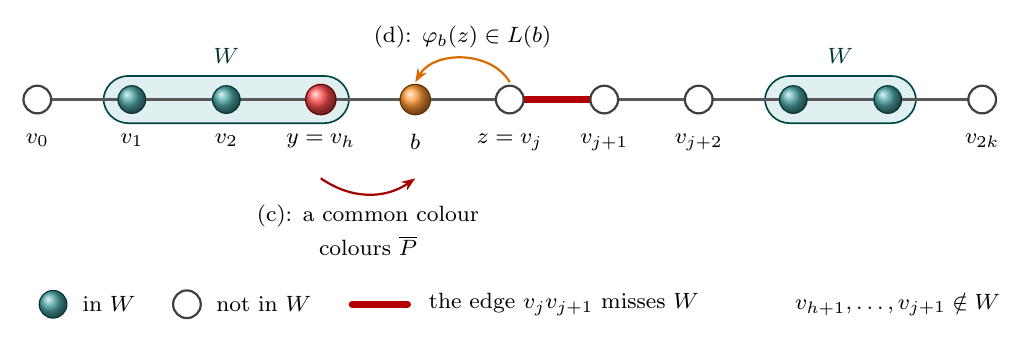
\includegraphics[width=0.95\textwidth]{figures/fig_key.png}
\caption{Step~(e) of the proof of Lemma~\ref{lem:key}. The shaded vertices form a minimal tight set $W$ and the edge $v_jv_{j+1}$ misses $W$. Either $b$ and $y$ share a colour, which gives a colouring by~(c), or their lists are complementary, and then the matching $\varphi_b$ gives $z$ a colour of $L(b)$, which $b$ can share with $z$ by~(d).}
\label{fig:key}
\end{figure}

\section{Unions of odd paths}\label{sec:path}

An \emph{odd linear forest} is a graph whose components are paths with an odd number of vertices. On a component $u_0u_1\cdots u_{2r}$ the vertices $u_0,u_2,\dots,u_{2r}$ are \emph{outer} and $u_1,u_3,\dots,u_{2r-1}$ are \emph{inner}. If $P$ has $p$ components, $s$ outer vertices and $t$ inner vertices, then $s=t+p$, so $t\le s-1$ when $P$ is nonempty. Two outer vertices are never adjacent in $P$, so the outer vertices form a clique of size $s$ in $\overline P$.

\begin{theorem}\label{thm:path}
Let $P$ be a nonempty odd linear forest with $s$ outer vertices, and let $L$ be a list assignment for $P$ with $|L(v)|\ge s-1$ for every vertex $v$. Then $\overline P$ is not $L$-colourable if and only if all outer vertices have the same list and this list has exactly $s-1$ colours.
\end{theorem}

\begin{proof}
If the outer vertices have a common list of $s-1$ colours, they cannot be coloured, since they form a clique of size $s$ in $\overline P$. We prove the converse by induction on the number of vertices. Let $P$, with vertex set $V$, $s$ outer and $t$ inner vertices, and $L$ be such that $\overline P$ is not $L$-colourable, and suppose that the converse holds for all odd linear forests with fewer vertices. Assume, for a contradiction, that the outer lists are not one common list of $s-1$ colours.

\smallskip\noindent\emph{Step 1: $\df(W)<\df(V)$ for every $W\subsetneq V$.} Let $X\subseteq V$ have the largest deficiency, and suppose that $X\ne V$. We first show that $\overline P[X]$ is $L$-colourable.

If some outer vertex $w$ is not in $X$, assign to every inner vertex $u$ an outer neighbour $\pi(u)\ne w$: on the component of $w$, the neighbour of $u$ on the side away from $w$, and on every other component, the neighbour of $u$ nearer to a fixed end of that component. Each outer vertex receives at most one inner vertex in this way, and $w$ receives none (Figure~\ref{fig:pairing}). The sets $X\cap(\{o\}\cup\pi^{-1}(o))$, for outer vertices $o\ne w$, cover $X$; there are at most $s-1$ of them, and each is a single vertex or the two ends of an edge of $P$. Lemma~\ref{lem:ert} with $q=s-1$ colours $\overline P[X]$.

If $X$ contains every outer vertex, then $P[X]$ is an odd linear forest with the same outer vertices as $P$, since deleting an inner vertex splits its path into two paths with an odd number of vertices whose outer vertices keep their positions. As $|X|<|V|$, the induction hypothesis and our assumption on the outer lists show that $\overline P[X]$ is $L$-colourable.

Let $f_X$ be an $L$-colouring of $\overline P[X]$, and put $L'(v)=L(v)\setminus L(X)$ for $v\in V\setminus X$. For $Z\subseteq V\setminus X$ the set $L(X\cup Z)$ is the disjoint union of $L(X)$ and $L'(Z)$, so $\df(X\cup Z)\le\df(X)$ gives $|L'(Z)|\ge|Z|$. By Lemma~\ref{lem:hall} there is an injective map $g$ on $V\setminus X$ with $g(v)\in L'(v)$. The colours of $g$ are distinct and avoid $L(X)$, so $f_X$ and $g$ together form an $L$-colouring of $\overline P$, a contradiction. Hence $V$ is the only set of largest deficiency, which is Step~1. Taking $W=\varnothing$ we obtain $\df(V)\ge1$, that is,
\begin{equation}\label{eq:LV}
|L(V)|\le|V|-1=s+t-1.
\end{equation}

\smallskip\noindent\emph{Step 2: $t\ge1$.} If $t=0$, then $|V|=s$ and every list is a subset of $L(V)$ with at least $s-1\ge|L(V)|$ colours, so every list equals $L(V)$ and has $s-1$ colours, contrary to our assumption.

\smallskip\noindent\emph{Step 3: any two lists meet.} Suppose that $L(u)\cap L(v)=\varnothing$ for some $u\ne v$. Then $2(s-1)\le|L(V)|\le s+t-1$ by~\eqref{eq:LV}, so $t\ge s-1$, and since $t=s-p\le s-1$ we get $t=s-1$ and $p=1$. Thus $P$ is a single path $v_0v_1\cdots v_{2k}$ with $k=s-1=t\ge1$, $|L(V)|=2k$, and $\df(V)=1$. By Step~1, $\df(W)\le0$, that is $|L(W)|\ge|W|$, for every $W\subsetneq V$. Every list has at least $k$ colours, so Lemma~\ref{lem:key} shows that $L(v_0)=L(v_2)=\dots=L(v_{2k})$ with $k=s-1$ colours, contrary to our assumption.

\smallskip\noindent\emph{Step 4: the two ends of a path.} By Step~2 some component $Q=u_0u_1\cdots u_{2r}$ has $r\ge1$, so its ends $u_0\ne u_{2r}$ are outer. By Step~3 there are colours $c\in L(u_0)\cap L(u_1)$ and $c'\in L(u_{2r})\cap L(u_{2r-1})$.

Let $P'=P-\{u_0,u_1\}$. It is an odd linear forest whose outer vertices are those of $P$ other than $u_0$, so it has $s-1\ge1$ of them. Put $L'(v)=L(v)\setminus\{c\}$, a list with at least $s-2$ colours. If $\overline{P'}$ had an $L'$-colouring, giving $c$ to $u_0$ and $u_1$ would extend it to an $L$-colouring of $\overline P$, since $u_0u_1$ is an edge of $P$. By the induction hypothesis the outer vertices of $P'$ have one common $L'$-list of $s-2$ colours. For an outer vertex $v\ne u_0$ the list $L(v)$ has at least $s-1$ colours, so $c\in L(v)$ and $L(v)=L'(v)\cup\{c\}$. Hence
\begin{equation}\label{eq:end0}
L(v)=S_0\ \text{for every outer vertex }v\ne u_0,\qquad\text{where }|S_0|=s-1\text{ and }c\in S_0.
\end{equation}
The same argument with $u_{2r}$, $u_{2r-1}$ and $c'$ shows that
\begin{equation}\label{eq:end1}
L(v)=S_1\ \text{for every outer vertex }v\ne u_{2r},\qquad\text{where }|S_1|=s-1.
\end{equation}
If $s\ge3$, there is an outer vertex $z\notin\{u_0,u_{2r}\}$, and $L(u_0)=S_1=L(z)=S_0=L(u_{2r})$ by~\eqref{eq:end1} and~\eqref{eq:end0}. If $s=2$, the outer vertices are $u_0$ and $u_{2r}$; the list $L(u_0)=S_1$ has one colour and contains $c$, and $L(u_{2r})=S_0$ has one colour and contains $c$, so $L(u_0)=L(u_{2r})=\{c\}$. In either case all outer vertices have one common list of $s-1$ colours, contrary to our assumption.
\end{proof}

\begin{figure}[ht]
\centering
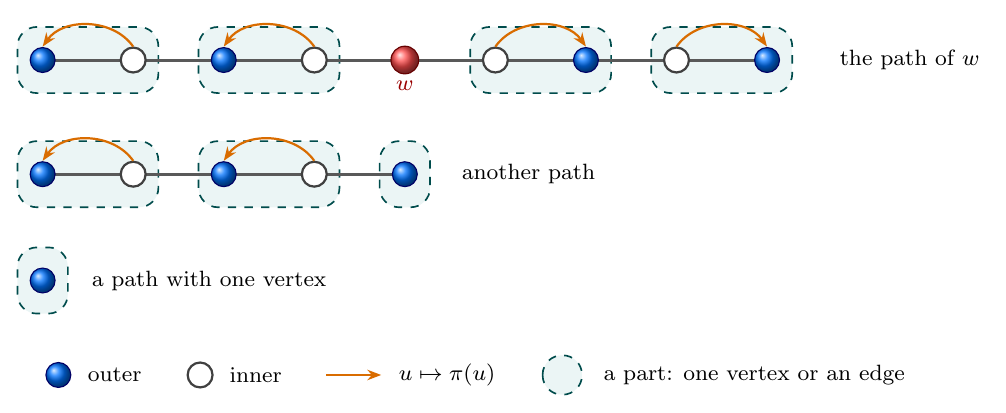
\includegraphics[width=0.95\textwidth]{figures/fig_pairing.png}
\caption{Step~1 of the proof of Theorem~\ref{thm:path}. Outer vertices are filled and inner vertices are hollow. Each inner vertex is sent to an outer neighbour other than $w$; on the path of $w$ it is sent away from $w$. The resulting parts (outlined) are single vertices or edges of $P$, and there are at most $s-1$ of them.}
\label{fig:pairing}
\end{figure}

\section{Odd cycles}\label{sec:cycle}

Let $m\ge2$ and let $C=v_0v_1\cdots v_{2m}v_0$ be the cycle of length $2m+1$; indices are taken modulo $2m+1$. The complement $\overline C$ is the odd antihole $\cbar{2m+1}$.

\begin{proposition}\label{prop:chi}
$\chi(\cbar{2m+1})=m+1$ for every $m\ge2$.
\end{proposition}

\begin{proof}
A colour class of $\overline C$ is a clique of $C$, and $C$ has no triangles, so every class has at most two vertices and at least $m+1$ colours are needed. The classes $\{v_{2i},v_{2i+1}\}$ for $0\le i<m$ and $\{v_{2m}\}$ form a colouring with $m+1$ colours.
\end{proof}

\begin{theorem}\label{thm:cycle}
Let $m\ge2$ and let $L$ be a list assignment for $\overline C$ with $|L(v)|\ge m$ for every vertex $v$. If $\overline C$ is not $L$-colourable, then all lists are equal.
\end{theorem}

\begin{proof}
Suppose that $\overline C$ is not $L$-colourable.

\smallskip\noindent\emph{Claim 1. Some two consecutive lists meet.} Otherwise the vertices whose lists contain a given colour are pairwise non-consecutive, so they form an independent set of $C$ and there are at most $m$ of them. As in the proof of Lemma~\ref{lem:ert}, $m|W|\le\sum_{w\in W}|L(w)|\le m|L(W)|$ for every set $W$ of vertices, and Lemma~\ref{lem:hall} gives an $L$-colouring of $\overline C$.

\smallskip\noindent\emph{Claim 2. If $c\in L(v_j)\cap L(v_{j+1})$, then $c\in L(v_{j+r})$ and $L(v_{j+r})=L(v_{j+2})$ for every even $r$ with $2\le r\le2m$.} The graph $C-\{v_j,v_{j+1}\}$ is the path $v_{j+2}v_{j+3}\cdots v_{j+2m}$ with $2m-1$ vertices, whose outer vertices are the $m$ vertices $v_{j+r}$ with $r$ even, $2\le r\le 2m$, and its complement is $\overline C-\{v_j,v_{j+1}\}$. Put $L'(v)=L(v)\setminus\{c\}$, a list with at least $m-1$ colours. An $L'$-colouring of this complement, together with the colour $c$ on $v_j$ and $v_{j+1}$, would be an $L$-colouring of $\overline C$. So Theorem~\ref{thm:path} with $s=m$ shows that the lists $L'(v_{j+r})$, $r$ even, are one common set of $m-1$ colours. Since $|L(v_{j+r})|\ge m$, each $L(v_{j+r})$ contains $c$ and equals $L'(v_{j+r})\cup\{c\}$. This proves Claim~2 (Figure~\ref{fig:cycle}).

\smallskip\noindent\emph{Conclusion.} By Claim~1 there are $j$ and $c$ with $c\in L(v_j)\cap L(v_{j+1})$. Write $L_r=L(v_{j+r})$. We apply Claim~2 four times, at the consecutive pairs starting at $v_j$, $v_{j-1}$, $v_{j+1}$ and $v_{j+2}$.
\begin{enumerate}
\item[(i)] At $v_j$: $c\in L_r$ and $L_r=L_2$ for even $r\in[2,2m]$. In particular $c\in L_{2m}=L_{-1}$ and $c\in L_2$.
\item[(ii)] At $v_{j-1}$, since $c\in L_{-1}\cap L_0$: $c\in L_r$ and $L_r=L_1$ for odd $r\in[1,2m-1]$. In particular $c\in L_3$, as $m\ge2$.
\item[(iii)] At $v_{j+1}$, since $c\in L_1\cap L_2$, with $r=2m$: $L_0=L_{1+2m}=L_3$.
\item[(iv)] At $v_{j+2}$, since $c\in L_2\cap L_3$, with $r=2m$: $L_1=L_{2+2m}=L_4$.
\end{enumerate}
By (iii) and (ii), $L_0=L_3=L_1$, and by (iv) and (i), $L_1=L_4=L_2$. So $L_0=L_1=L_2$, and by (i) and (ii) every list equals $L_1$ or $L_2$.
\end{proof}

\begin{figure}[ht]
\centering
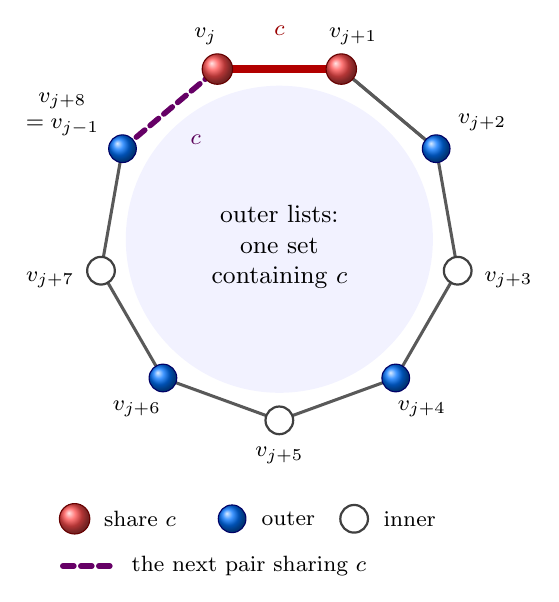
\includegraphics[width=0.62\textwidth]{figures/fig_cycle.png}
\caption{Claim~2 in the proof of Theorem~\ref{thm:cycle} for $m=4$. The consecutive vertices $v_j$ and $v_{j+1}$ share the colour $c$. The rest of the cycle is a path whose outer vertices $v_{j+2},v_{j+4},\dots,v_{j+2m}$ (filled) then all carry one list containing $c$. Since $v_{j+2m}=v_{j-1}$, the colour $c$ passes to the pair $v_{j-1}v_j$, and the claim applies again.}
\label{fig:cycle}
\end{figure}

\begin{proof}[Proof of Theorem~\ref{thm:main}]
Put $m=\ell-1\ge2$, so that $\cbar{2\ell-1}=\overline C$. By Proposition~\ref{prop:chi}, $\chi(\overline C)=\ell$. Let $L$ be a list assignment in which every list has at least $\ell-1=m$ colours and suppose that $\overline C$ is not $L$-colourable. By Theorem~\ref{thm:cycle} all lists are one set $S$. If $|S|\ge\ell$, a colouring of $\overline C$ with $\ell$ colours from $S$ would be an $L$-colouring, so $|S|=\ell-1$. In particular every $(\ell-1)$-assignment from which $\overline C$ cannot be coloured is constant, and $\cbar{2\ell-1}$ is strongly $\ell$-chromatic-choosable.
\end{proof}

\section{Odd antiholes in critical graphs}\label{sec:critical}

We now deduce Corollary~\ref{cor:conj3}. The argument is that of Fiujlaali and McDonald~\cite[Theorem~10]{FM}, with Theorem~\ref{thm:main} in place of Conjecture~\ref{conj:9}; we give it in full so that the proof is complete.

\begin{proof}[Proof of Corollary~\ref{cor:conj3}]
Let $A$ be an odd antihole of length $2\ell-1$ in $G$, where $\ell=\Delta-k+4$; an odd antihole has length at least five, so $\ell\ge3$. Suppose that $G\ne A$. Since $A$ is an induced subgraph of $G$, there is a vertex $v\notin V(A)$. Since $A$ is a subgraph of $G-v$, criticality gives $\ell=\chi(A)\le\chi(G-v)\le k-1$. Put $q=k-\ell\ge1$, so that
\[
k=\ell+q\qquad\text{and}\qquad \Delta=2\ell+q-4.
\]
By criticality $G-V(A)$ has a proper colouring $\varphi$ with a set $P$ of $k-1=\ell+q-1$ colours. For $v\in V(A)$ let $L(v)=P\setminus\varphi(N(v)\setminus V(A))$. Each vertex of $A$ has $2\ell-4$ neighbours in $A$, hence at most $\Delta-(2\ell-4)=q$ neighbours outside $A$, and $|L(v)|\ge\ell-1$. An $L$-colouring of $A$ would extend $\varphi$ to a proper colouring of $G$ with $k-1$ colours, so by Theorem~\ref{thm:main} all the lists $L(v)$ are one set $S$ of $\ell-1$ colours.

Let $F=P\setminus S$, so $|F|=q$. Every $v\in V(A)$ has a neighbour outside $A$ of each colour in $F$ and at most $q$ neighbours outside $A$. Hence $v$ has exactly one outside neighbour $z_v(c)$ of each colour $c\in F$, and no outside neighbour with a colour in $S$.

Fix $c\in F$ and $a\in S$, and consider the components of the subgraph of $G-V(A)$ induced by the vertices of colours $a$ and $c$. Suppose that one of these components, $B$, contains $z_x(c)$ but not $z_y(c)$ for some $x,y\in V(A)$. Exchanging $a$ and $c$ on $B$ gives a proper colouring $\varphi'$ of $G-V(A)$. The only outside neighbour of a vertex $v\in V(A)$ whose colour is $a$ or $c$ is $z_v(c)$, so the new lists are $(S\setminus\{a\})\cup\{c\}$ when $z_v(c)\in B$ and $S$ otherwise. These are $(\ell-1)$-sets and they are not all equal, so Theorem~\ref{thm:main} colours $A$ from them, and $G$ is $(k-1)$-colourable, a contradiction. Hence all the vertices $z_v(c)$, $v\in V(A)$, lie in one component $B$.

Suppose next that $z_x(c)\ne z_y(c)$ for some $x,y\in V(A)$. The antihole $A$ is connected, so we may take $x$ and $y$ adjacent. Let $T=t_0t_1\cdots t_{2h}$ be a shortest path in $B$ from $t_0=z_x(c)$ to $t_{2h}=z_y(c)$; its vertices alternate between the colours $c$ and $a$, so its length $2h$ is even and positive. A chord $t_it_j$ of $T$ would join vertices of different colours, so it would be an edge of $B$ and would shorten $T$; hence $T$ is an induced path. The vertex $x$ has no outside neighbour of colour $a$ and exactly one of colour $c$, so $t_0$ is its only neighbour on $T$; likewise $t_{2h}$ is the only neighbour of $y$ on $T$. Then $x\,t_0t_1\cdots t_{2h}\,y\,x$ is an induced cycle of odd length $2h+3\ge5$, an odd hole in $G$, a contradiction. So for each $c\in F$ there is one vertex $z_c$ adjacent to every vertex of $A$.

The set $Z=\{z_c:c\in F\}$ has $q$ elements, and $N(v)\setminus V(A)=Z$ for every $v\in V(A)$. Every $z\in Z$ has $2\ell-1$ neighbours in $A$, so
\[
d_{G-V(A)}(z)\le\Delta-(2\ell-1)=q-3,
\]
and in particular $q\ge3$. Let $R=G-(V(A)\cup Z)$, keep the colouring $\varphi$ on $R$, and choose a set $Q\subseteq P$ of $q-1$ colours. For $z\in Z$ let $M(z)=Q\setminus\varphi(N(z)\cap V(R))$. Then
\[
|M(z)|\ge q-1-d_R(z)\ge q-1-\bigl(q-3-d_{G[Z]}(z)\bigr)=d_{G[Z]}(z)+2,
\]
so $G[Z]$ can be coloured greedily from the lists $M(z)$. This gives a proper colouring of $G-V(A)$ in which $Z$ uses only colours of $Q$. Every vertex of $A$ has outside neighbourhood $Z$, so the $\ell$ colours of $P\setminus Q$ are available at every vertex of $A$, and since $\chi(A)=\ell$ the colouring extends to $G$ with $k-1$ colours. This contradicts $\chi(G)=k$, so $G=A$.
\end{proof}

\section*{Declarations}

\subsection*{Funding} No funding was received for this work.

\subsection*{Conflict of interest} The authors declare no conflict of interest.

\subsection*{Data availability} The proofs in this paper are complete by hand. The source of the paper and programs that check Theorem~\ref{thm:main} for $\ell=3$ and $\ell=4$, by examining every assignment of lists of size $\ell-1$ up to renaming the colours, are in release \texttt{v2.0.0} of the repository named in the note under the abstract, archived as \href{https://doi.org/10.5281/zenodo.23663712}{10.5281/zenodo.23663712}; the paper does not depend on them.

\begingroup\sloppy\emergencystretch=3em\hbadness=5000
\begin{thebibliography}{99}

\bibitem{BKMS}
A.~Bernshteyn, H.~Kaul, J.~A.~Mudrock and G.~Sharma, On strongly and robustly critical graphs, J. Graph Theory 112 (2026), no.~4, 469--483. \href{https://doi.org/10.1002/jgt.70033}{doi:10.1002/jgt.70033}.

\bibitem{Bha22a}
D.~Bhattacharjee, Establishing equivariant class $[O]$ for hyperbolic groups, Asian Res. J. Math. 18 (2022), no. 11, 362--369. \href{https://doi.org/10.9734/arjom/2022/v18i11615}{doi:10.9734/arjom/2022/v18i11615}.

\bibitem{Bha22b}
D.~Bhattacharjee, Non-commutativity over canonical suspension $\eta$ for genus $g\ge1$ in hypercomplex structures for potential $\rho\phi$, Asian Res. J. Math. 18 (2022), no. 11, 332--341. \href{https://doi.org/10.9734/arjom/2022/v18i11607}{doi:10.9734/arjom/2022/v18i11607}.

\bibitem{BB26}
D.~Bhattacharjee, U.~Bhattacharya, Iterated nerve complexes for $k$-fold sensor coverage, Preprints.org (2026). \href{https://doi.org/10.20944/preprints202606.1351.v2}{doi:10.20944/preprints202606.1351.v2}.

\bibitem{CLLZ}
R.~Chen, K.~Lan, X.~Lin and Y.~Zhou, The chromatic number of odd-hole-free graphs, Discrete Appl. Math. 370 (2025), 84--87. \href{https://doi.org/10.1016/j.dam.2025.02.043}{doi:10.1016/j.dam.2025.02.043}.

\bibitem{CRST}
M.~Chudnovsky, N.~Robertson, P.~Seymour and R.~Thomas, The strong perfect graph theorem, Ann. of Math. (2) 164 (2006), no.~1, 51--229. \href{https://doi.org/10.4007/annals.2006.164.51}{doi:10.4007/annals.2006.164.51}.

\bibitem{ERT}
P.~Erd\H{o}s, A.~L.~Rubin and H.~Taylor, Choosability in graphs, in: Proceedings of the West Coast Conference on Combinatorics, Graph Theory and Computing (Arcata, 1979), Congr. Numer. 26, Utilitas Math., Winnipeg, 1980, pp.~125--157.

\bibitem{FM}
A.~Fiujlaali and J.~McDonald, Restricting odd antiholes in critical graphs via list coloring, preprint, \href{https://arxiv.org/abs/2610.14241}{arXiv:2610.14241} (2026).

\bibitem{GMS}
R.~Galindo, J.~McDonald and S.~Shan, Cliques and high odd holes in graphs with chromatic number equal to maximum degree, Discrete Appl. Math. 383 (2026), 383--386. \href{https://doi.org/10.1016/j.dam.2026.01.014}{doi:10.1016/j.dam.2026.01.014}.

\bibitem{Hall}
P.~Hall, On representatives of subsets, J. London Math. Soc. 10 (1935), 26--30. \href{https://doi.org/10.1112/jlms/s1-10.37.26}{doi:10.1112/jlms/s1-10.37.26}.

\bibitem{KM}
H.~Kaul and J.~A.~Mudrock, Criticality, the list color function, and list coloring the Cartesian product of graphs, J. Comb. 12 (2021), no.~3, 479--514. \href{https://doi.org/10.4310/JOC.2021.v12.n3.a4}{doi:10.4310/\allowbreak JOC.2021.v12.n3.a4}.

\bibitem{NRW}
J.~A.~Noel, B.~A.~Reed and H.~Wu, A proof of a conjecture of Ohba, J. Graph Theory 79 (2015), no.~2, 86--102. \href{https://doi.org/10.1002/jgt.21819}{doi:10.1002/jgt.21819}.

\bibitem{Ohba}
K.~Ohba, On chromatic-choosable graphs, J. Graph Theory 40 (2002), no.~2, 130--135. \href{https://doi.org/10.1002/jgt.10033}{doi:10.1002/jgt.10033}.

\bibitem{STV}
M.~Stiebitz, Z.~Tuza and M.~Voigt, On list critical graphs, Discrete Math. 309 (2009), no.~15, 4931--4941. \href{https://doi.org/10.1016/j.disc.2008.05.021}{doi:10.1016/j.disc.2008.05.021}.

\end{thebibliography}
\endgroup

\end{document}
